\chapter{Восстановление функции распределения убегающих электронов по измеренному спектру жёсткого рентгеновского излучения}
\label{ch:ch3}

% ==========================================================

\section{Восстановление исходного спектра гамма излучения по измеренному спектру}

В ходе применения описанных в главе~\ref{ch:ch2} процедур из записанной с помощью АЦП осциллограммы можно получить массив данных <<время-амплитуда>>, на основании которого построить спектр зарегистрированных событий. Однако полученный таким образом спектр не является спектром гамма-излучения, испущенным источником гамма квантов. 

Задача восстановления исходного распределения является весьма актуальной при обработке спектров и изображений в астрофизике~\cite{JungRichardt2016}, биологии и медицине~\cite{Vardi1985}, гамма и рентгеновской спектроскопии. Попытки восстановления исходного энергетического распределения из спектров, измеренных сцинтилляционными и полупроводниковыми детекторами, проводились ранее, например, в работах~\cite{Raad2008,Meng2000} и других.

Актуальность задачи привела к созданию большого числа различных методов деконволюции спектров и изображений. В ряде работ, например~\cite{Meng2000,Lanteri1999,Morhac2011,Jeffrey1986,Bouchet1995}, производилось сравнение между различными методами с целью выбрать наиболее подходящий для обработки спектров. Показано, что метод максимальной вероятной оценки с использованием ожидаемой максимизации (maximum likelihood estimation using expectation maximization, ML-EM)~\cite{Vardi1985}, известный так же как метод Ричардсона-Луси~\cite{Richardson1972,Lucy1974}, является одним из лучших при восстановлении гамма спектров: он демонстрирует хорошую устойчивость к шумам исходных данных и позволяет сравнительно точно восстанавливать исходные спектры~\cite{Meng2000,Morhac2011}.

Во всех упомянутых работах методы деконволюции применялись к случаю, когда исходный спектр является дискретным. Кроме того, предполагалась большая статистика спектров. В то же время спектры, получаемые в экспериментах на токамаках, обычно имеют весьма малую статистику~(\cite{Khilkevitch2013,Shevelev2018,Reux2022,Chugunov2011,Shevelev2013} и другие). Помимо этого, в спектрах зачастую присутствует вклад нейтронного излучения. Спектры жёсткого рентгеновского излучения, генерируемые убегающими электронами, почти всегда имеют непрерывный характер~\cite{Shevelev2013}. Всё это усложняет применение описанных выше алгоритмов к экспериментальным данным.~\cite{Khilkevitch2013} 

В этой главе описаны методы, с помощью которых возможно на основе измененных амплитудных спектров событий, зарегистрированных с помощью детекторов, восстановить энергетические спектры гамма излучения; кроме того, будет описано применение методов для восстановления функции распределения убегающих электронов по энергии.

% ==========================================================

\section{ Восстановление спектра гамма излучения по измеренному спектру излучения }

% ----------------------------------------------------------

\subsection{ Использование метода ML-EM для восстановления спектра излучения }

Измеренный с помощью гамма детектора спектр $s(\varepsilon)$ может быть представлен в следующем виде:
\begin{equation}
  \label{eq:BaseConvolution}
  s(\varepsilon) = \int \limits_0^{+\infty} g( \varepsilon' ) h( \varepsilon, \varepsilon' ) d \varepsilon' + n(\varepsilon)
\end{equation}
где $g(\varepsilon)$ --- спектр гамма излучения от источника излучения, $n(\varepsilon)$ --- статистический пуассоновский шум, $ h( \varepsilon, \varepsilon' ) $ --- передаточная функция, $\varepsilon$ --- энергия. Задача восстановления заключается в нахождении спектра гамма излучения $g$ по измеренному спектру $s$ при известной передаточной функции $h$.~\cite{Khilkevitch2013}

Для решения уравнения~\ref{eq:BaseConvolution} необходимо знать функцию $ h( \varepsilon, \varepsilon' ) $. Это --- передаточная функция, её физический смысл следующий: для моноэнергетического пучка гамма квантов с энергией $\varepsilon'$, испускаемый источником, с помощью детектора будет зарегистрирован спектр, равный $s(\varepsilon) = h(\varepsilon, \varepsilon') \cdot N_{\gamma}$ без учёта шума, где $N_{\gamma}$ --- количество гамма квантов, испущенных источником. Передаточная функция $h$ зависит от характеристик самого детектора (площади, материала, эффективности, относительного влияния на зарегистрированный спектр таких эффектов как комптоновское рассеяние, интенсивности пиков полного поглощения, одиночного и двойного вылета, и тому подобное), от процессов, произошедших с квантом после его испускания на пути к детектору (поглощение в конструкциях, размещённых на пути гамма кванта от источника к детектору, отражение от окружающих конструкций, и так далее), от распределения испускаемого излучения по углам и от геометрического расположения детектора относительно источника гамма квантов. Функция $h$ может быть измерена экспериментально, однако на практике проще получить её с помощью численного моделирования с помощью одного из кодов, например с помощью компьютерного кода MCNP (Monte Carlo N-Particle code) и программы MCAM (Monte Carlo Automatic Modeling Program for Radiation Transport Simulation)~\cite{Hendricks2004,Fischer2005,Wu2009}.

Задачи определения неизвестного $x$ вида 
\begin{equation*}
  y = A x, x \in X, y \in Y
\end{equation*}
где $X$ и $Y$ --- некоторые пространства, $A$ --- оператор: $ A : X \rightarrow Y $, называются корректными по Адамару, если для каждого фиксированного $y$ решение $x$ существует, единственно и устойчиво. Под устойчивостью тут подразумевается то, что при малом изменении $y$ значение решения $x$ так же изменится мало~\cite{Liskovets1982}. Решение уравнения~\ref{eq:BaseConvolution} представляет собой некорректно поставленную по Адамару задачу, близкую к задаче деконволюции. Для решения подобного класса задач известен целый ряд методов, часть из которых могут быть применены и в задачах гамма-спектрометрии.

Уравнение~\ref{eq:BaseConvolution} можно переписать в дискретной форме:
\begin{equation}
  \label{eq:BaseConvolutionMatrix}
  s = H \cdot g + n 
\end{equation}
где $s$, $g$, $n$ --- вектора, $H$ --- матрица. Для выбранной дискретной сетке по энергиям размерностью $N$ в интервале $ \varepsilon_0 \ldots \varepsilon_N $ элементы векторов оказываются равными значениям
\begin{equation*}
  s_i = \int \limits_{\varepsilon_i}^{\varepsilon_{i+1}} s( \varepsilon' ) d \varepsilon'
\end{equation*}
Для простоты можно считать, что эта сетка одинаковая для измеренного спектра и исходного спектра гамма излучения, но в общем случае это может быть и не так

Метод ML-EM \cite{Vardi1985,Richardson1972,Lucy1974} может быть применён для решения уравнений вида \ref{eq:BaseConvolutionMatrix}.~\cite{Khilkevitch2013,Shevelev2013} Это итеративный алгоритм, на каждой итерации следующее значение вычисляется как
\begin{equation*}
  g_i^{p+1} = g_i^p \cdot \sum \limits_{j = 0 }^{N} h_{j,i} \frac{ s_j }{ \sum \limits_{k=0}^{N} h_{j,k} g_k^p }
\end{equation*}
где верхний индекс $p$ --- номер итерации. На каждом шаге алгоритма выполняется преобразование 
\begin{equation*}
  g_i^p = \max \left( g_i^p, 0 \right)
\end{equation*}
которое обеспечивает неотрицательность решения --- очевидно, что искомая интенсивность гамма излучения не может быть отрицательной. В качестве начального приближения для работы алгоритма можно использовать значение
\begin{equation*}
  g^0 = \frac{ s }{ \| H s \| }
\end{equation*}
где $ \| H s \| $ --- норма вектора $ H s $. Условие для окончания работы алгоритма можно задать следующим образом:
\begin{equation*}
  \| s - H g^{p-1} \| - \| s - H g^p \| < \epsilon \cdot N
\end{equation*}
где $\epsilon$ --- параметр алгоритма.~\cite{Shevelev2013} 

Базовый алгоритм может быть модифицирован. В задачах гамма-диагностики о функции $g$ обычно имеется хотя бы минимальная априорная информация. Так, для спектра излучения, который образуется в результате ядерных реакций, присутствует ряд дискретных линий. Эти линии могут быть уширены за счёт доплеровского уширения линий. Для такого спектра можно использовать процедуру, основанную на работе~\cite{Morhac2011} и модифицированную в~\cite{Khilkevitch2013,Shevelev2013}: на каждом k-том шаге проводить <<вытягивание>> линий с помощью процедуры
\begin{equation*}
  g^{p, boost}_i = \left( g^p_i \right)^{\beta} \cdot \frac{ \sum_j g^p_i }{ \sum_j g^{p, boost}_j }
\end{equation*}
где значение степени $\beta$ --- параметр алгоритма, он должен быть чуть больше 1.0 (например, 1.01). 

Спектр излучения, генерируемого убегающими электронами, обычно имеет непрерывный характер. В это случае предлагается использовать другую модификацию: на каждом l-ом шаге сглаживать полученное решение. Можно использовать линейное сглаживание с весом:
\begin{equation*}
  g^{p, smooth}_i = w \cdot \left( g^p_{i-1} + g^p_i + g^p_{i+1} \right)/3 + ( 1 - w ) \cdot g^p_i
\end{equation*}
где коэффициент $w$ --- параметр алгоритма. Тут использовано сглаживание по трём точкам, но аналогично можно использовать линейное сглаживание по пяти или семи точкам, или другие способы сглаживания.~\cite{Khilkevitch2013} При линейном сглаживании необходимо обратить внимание на следующую особенность функции отклика $h$, используемую при восстановлении функции распределения убегающих электронов: электроны с энергией $\varepsilon_e$ генерируют гамма кванты с энергией преимущественно $\varepsilon_{\gamma} \ll \varepsilon_e$. Это приводит к тому, что значение вектора $g_i$ определяется с очень большой ошибкой при малых значениях индекса $i$; а процедура сглаживания приводит к нежелательному распространению этой ошибки в область больших энергий. Для того, чтобы этого избежать, в некоторых случаях имеет смысл сглаживать промежуточное решение только начиная с некоторого $i_{smooth} > 0$, значение которого --- параметр алгоритма (обычно в районе 10--20)~\cite{Khilkevitch2013}.

В случае, если искомая функция $g$ имеет смешанный характер, то есть содержит как гладкую непрерывную часть, так и дискретные пики, восстановление становится особенно сложным, поскольку решение имеет тенденцию к осцилляциям. В этом случае приходится эврестически подбирать параметры выполнения процедуры восстановления.

Для определения ошибок определения амплитуды может быть применён метод Монте-Карло~\cite{Shirk1985}. Для этого генерируется $M$ наборов векторов 
\begin{equation*}
  {{s'}_i}^{m} = R^{psn}(s_i)
\end{equation*}
где $ R^{psn}(x) $ --- случайное число с пуассоновским распределением и среднем значением $x$. Затем для каждого вектора ${s'}^{m}$ ищется соответствующее ему решение ${g'}^{m}$ с помощью описанного выше алгоритма ML-EM. Затем ищутся величины
\begin{equation*}
  \Delta_i = \sqrt{ \frac{1}{M} \sum \limits_{ m = 0 }^{M} \left( {g'_i}^{m} - g_i \right)^2 }
\end{equation*}
которые представляют собой среднеквадратичные отклонения для найденного решения $g$.~\cite{Shevelev2013}

Описанный выше алгоритм реализован в программном коде <<DeGaSum>>.~\cite{Khilkevitch2013}

% ----------------------------------------------------------

\subsection{ Проверка корректности восстановления и отработка методики для калибровочных источников излучения }

Для проверки корректности было проведено несколько экспериментов в лабораторных условиях с использованием калибровочных источников с известной интенсивностью излучения. 

В первом эксперименте использовались источники ${}^{60}$Co и ${}^{137}$Cs. Для восстановления спектра необходимо предварительно провести расчеты аппаратных функций детектора с реалистичными геометрическими и техническими параметрами в широком диапазоне энергий с как можно меньшими шагами по энергии, а так же рассчитать эффекты, возникающие при движении гамма кванта к детектору. Примеры аппаратных функций сцинтилляционного детектора, рассчитанных по программе MCNP (Monte-Carlo N-Particle), представлены на рисунке~\ref{fig:mcnpInstFunctionsNaI}; расчёты выполнял А.~Е.~Шевелев. Расчёты проводились для коллимированного пучка гамма-излучения. Полученные спектры нормировались на число гамма-квантов, вышедших из модельного источника, и ширину шага по энергии. В спектрах можно увидеть большие пики полного поглощения энергии, более мелкие пики одинарного вылета и непрерывные участки, соответствующие комптоновскому рассеянию гамма-излучения. Пики двойного вылета очень малы из-за большого размера и высокой эффективности сцинтилляционного кристалла. Моделирование проводилось для детектора NaI(Tl) размером $\varnothing$127$\times$152~мм с энергетическим разрешением 7\% на линии 662~кэВ. Использование детектора NaI(Tl) обусловлено желанием проверить алгоритм в более сложных условиях, используя детектор с заведомо низким разрешением по сравнению с более современными детекторами LaBr3(Ce).

\begin{figure}[ht!]
  \centerfloat{ 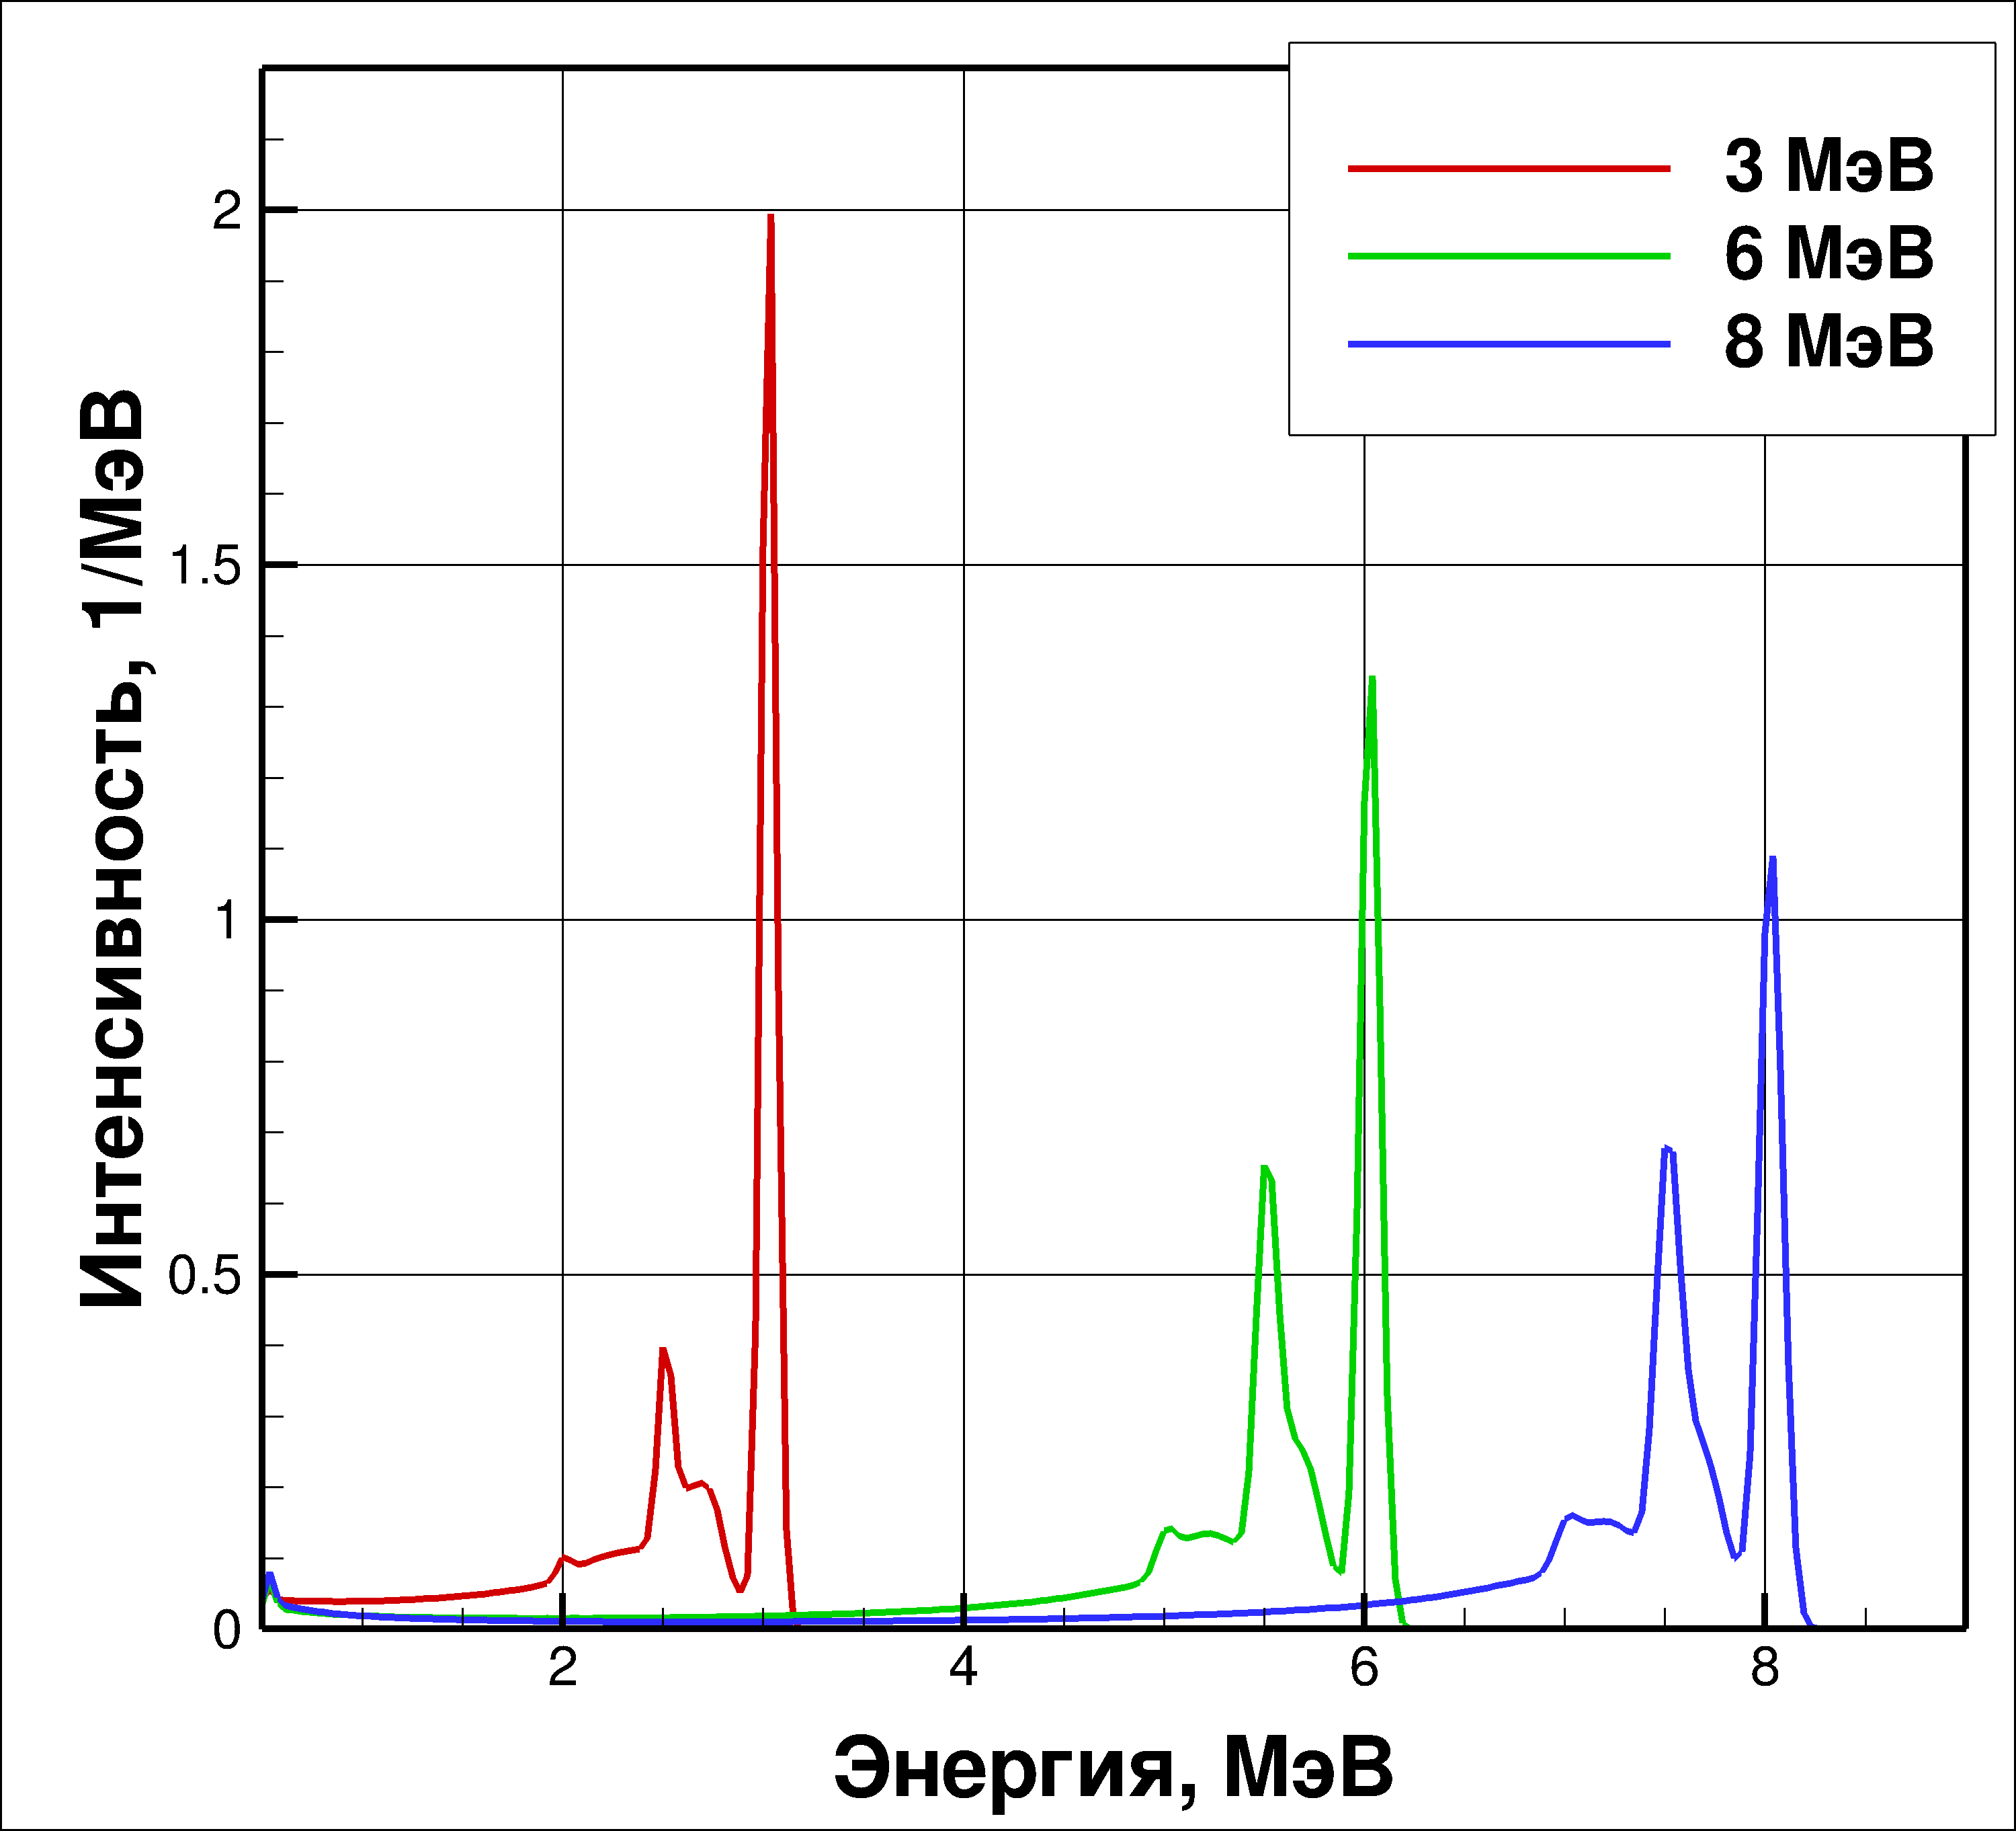
\includegraphics[width=0.52\linewidth]{mcnpInstFunctionsNaI} }
  \caption{ Примеры аппаратных функций, рассчитанных с помощью кода MCNP для детектора NaI(Tl) для различных значений энергии поглощаемых гамма квантов.~\cite{Shevelev2013} }
  \label{fig:mcnpInstFunctionsNaI}
\end{figure}

Были проведены измерения с использованием детектора NaI(Tl) размером $\varnothing$150$\times$100~мм с энергетическим разрешением 11,5\% на линии 661.6~кэВ. Функции отклика этого детектора рассчитывались по программе MCNP в диапазоне энергий 60--3000~кэВ с шагом 20~кэВ; расчёты выполнял А.~Е.~Шевелев. В разработанной расчетной модели источник изотропного гамма-излучения располагался на расстоянии 25.5~см от детектора. На одинаковом расстоянии от реального детектора для проведения измерений были установлены радиоактивные источники ${}^{60}$Co и ${}^{137}$Cs с известной активностью распада. Результаты обработки измеренного спектра показаны на рисунке~\ref{fig:cocsReconstructIoffe}. Время набора первого спектра составляет 150~секунд, время набора второго спектра --- 2~секунды, оба спектра были набраны в одинаковой геометрии. Обработка второго спектра иллюстрирует способность алгоритма работать с данными с низкой статистикой. Количество событий в восстановленных пиках соответствует количеству гамма-квантов, испущенных радиоактивными источниками во время регистрации спектра. Применяемая методика позволила определить активность радиоактивных источников с точностью 1.5\% для спектра с временем набора 150~секунд и 2.4\% для спектра с временем набора 2~секунды.~\cite{Shevelev2013}

\begin{figure}[ht!]
    \begin{minipage}[b][][b]{0.95\linewidth}\centering
        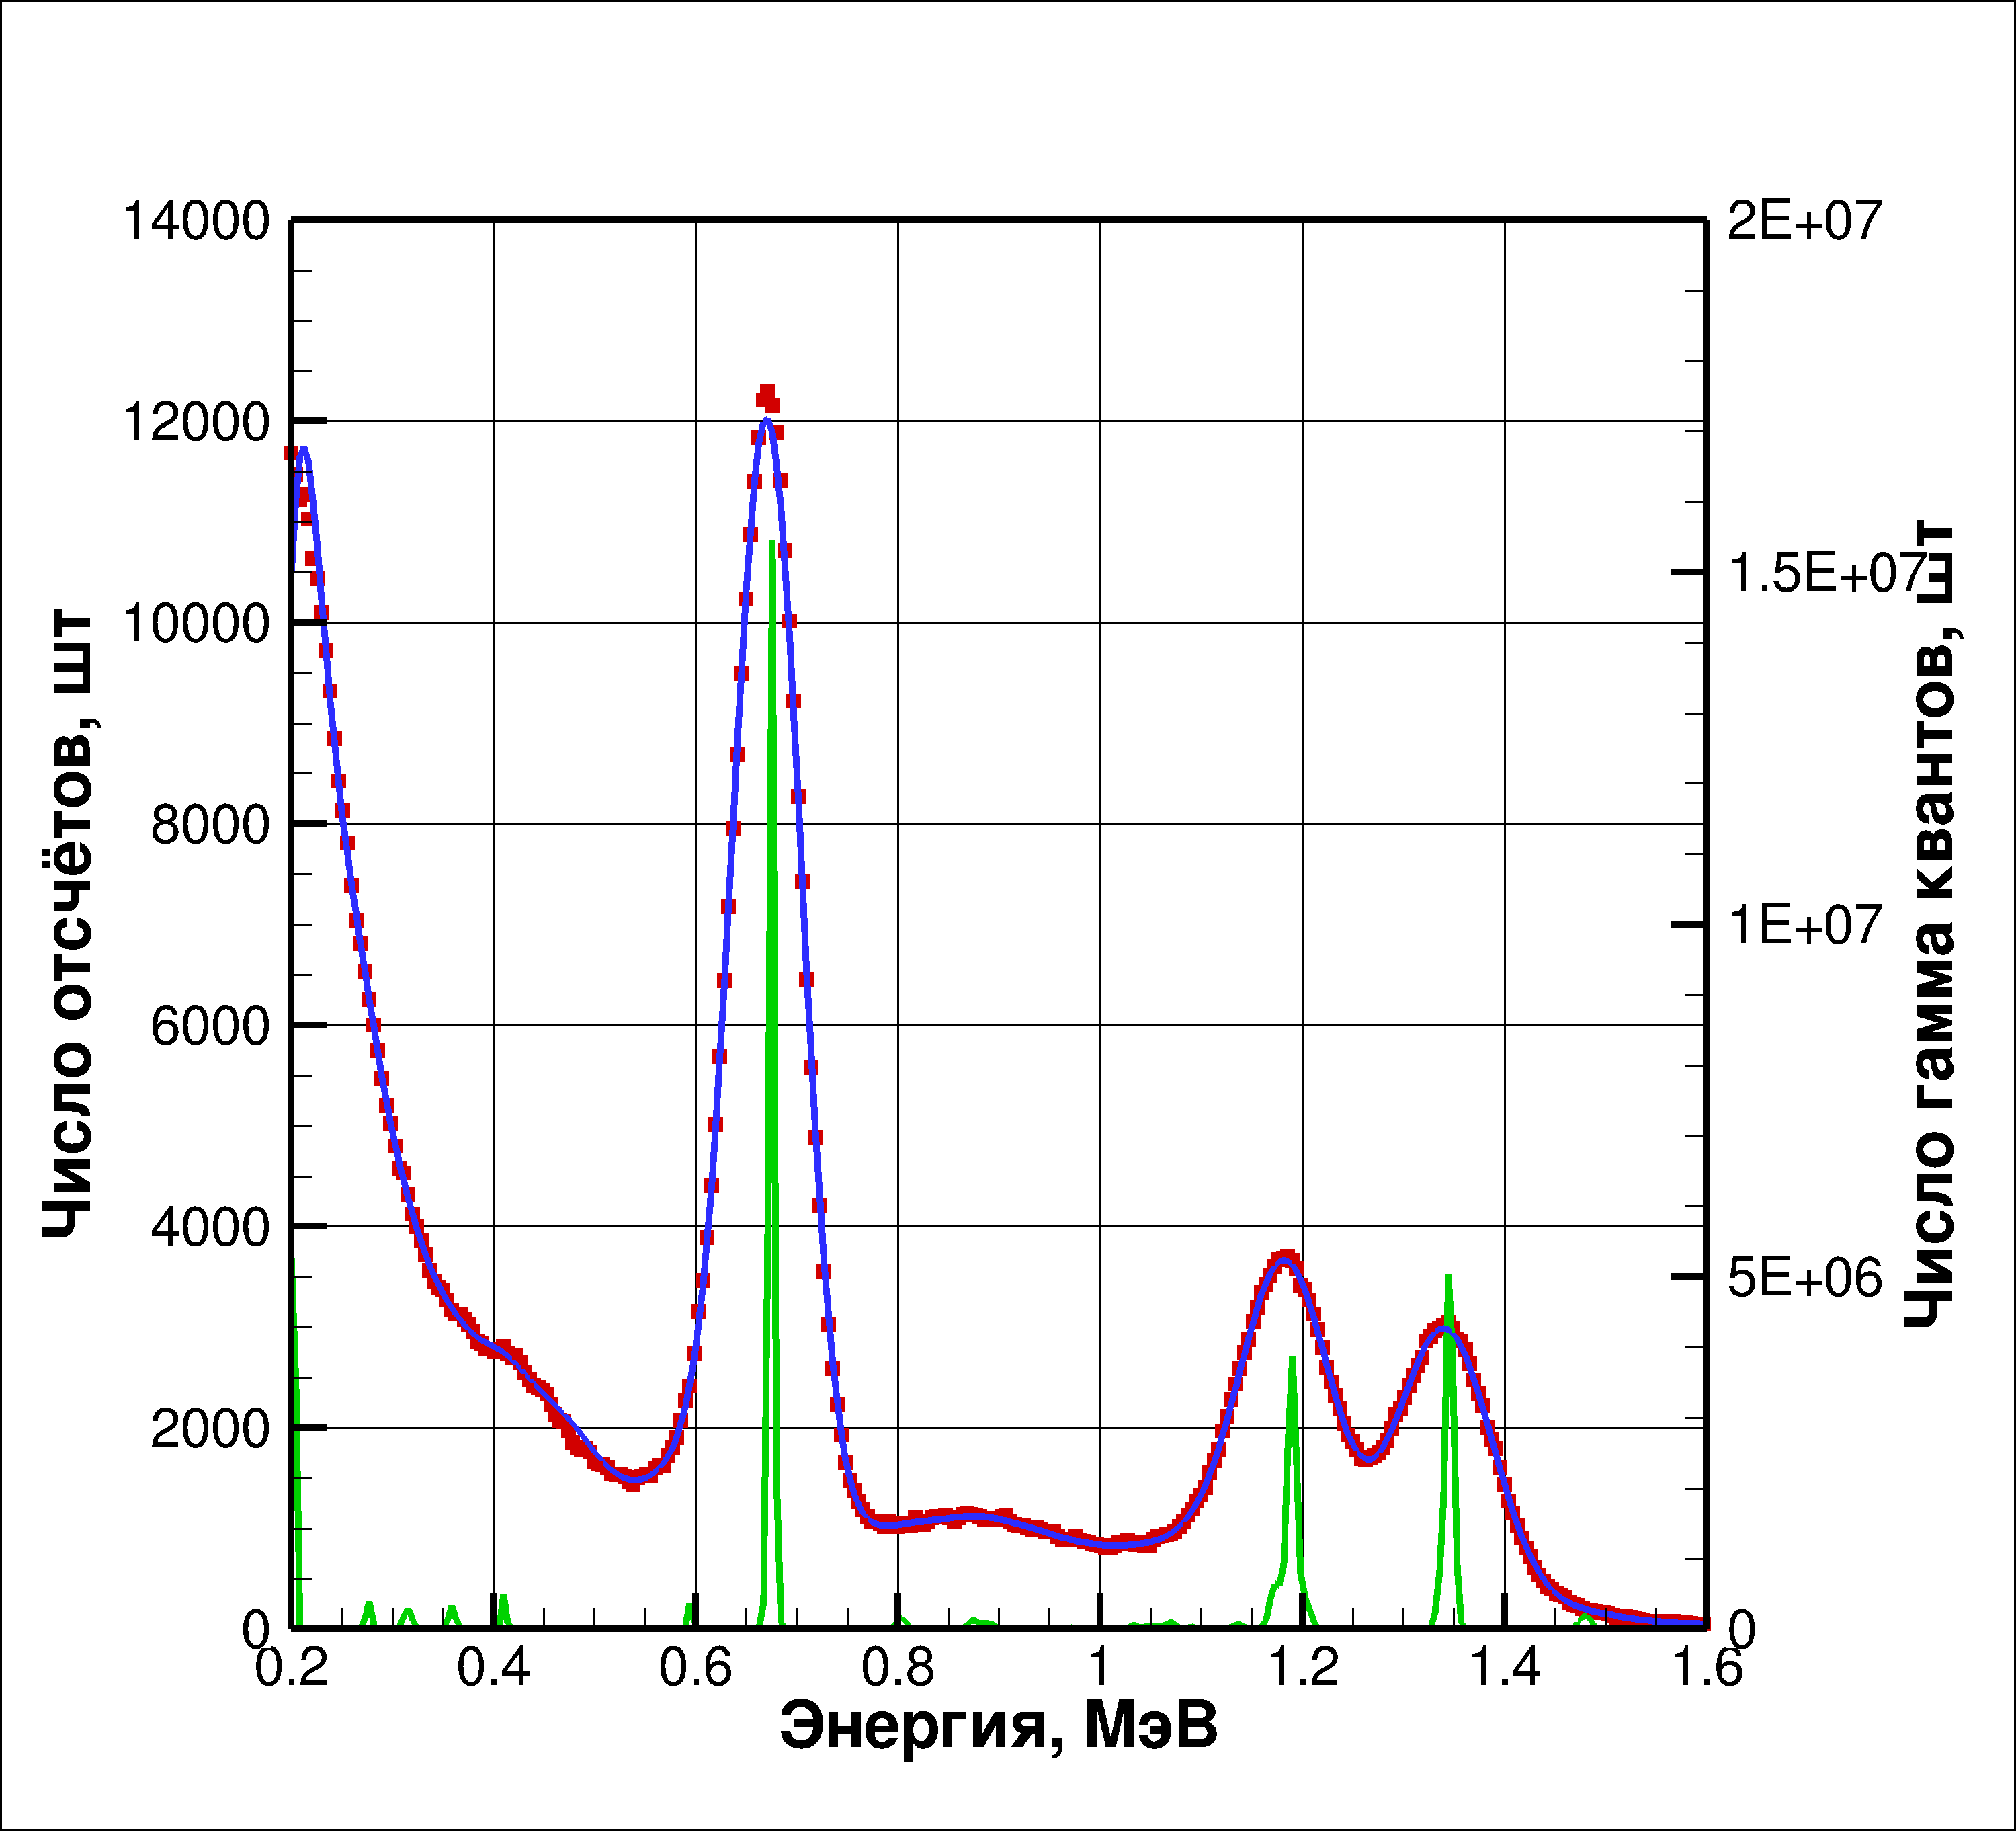
\includegraphics[width=0.52\linewidth]{cocsReconstructIoffe300s} \\ а) \\
    \end{minipage}
    \vfill
    \begin{minipage}[b][][b]{0.95\linewidth}\centering
        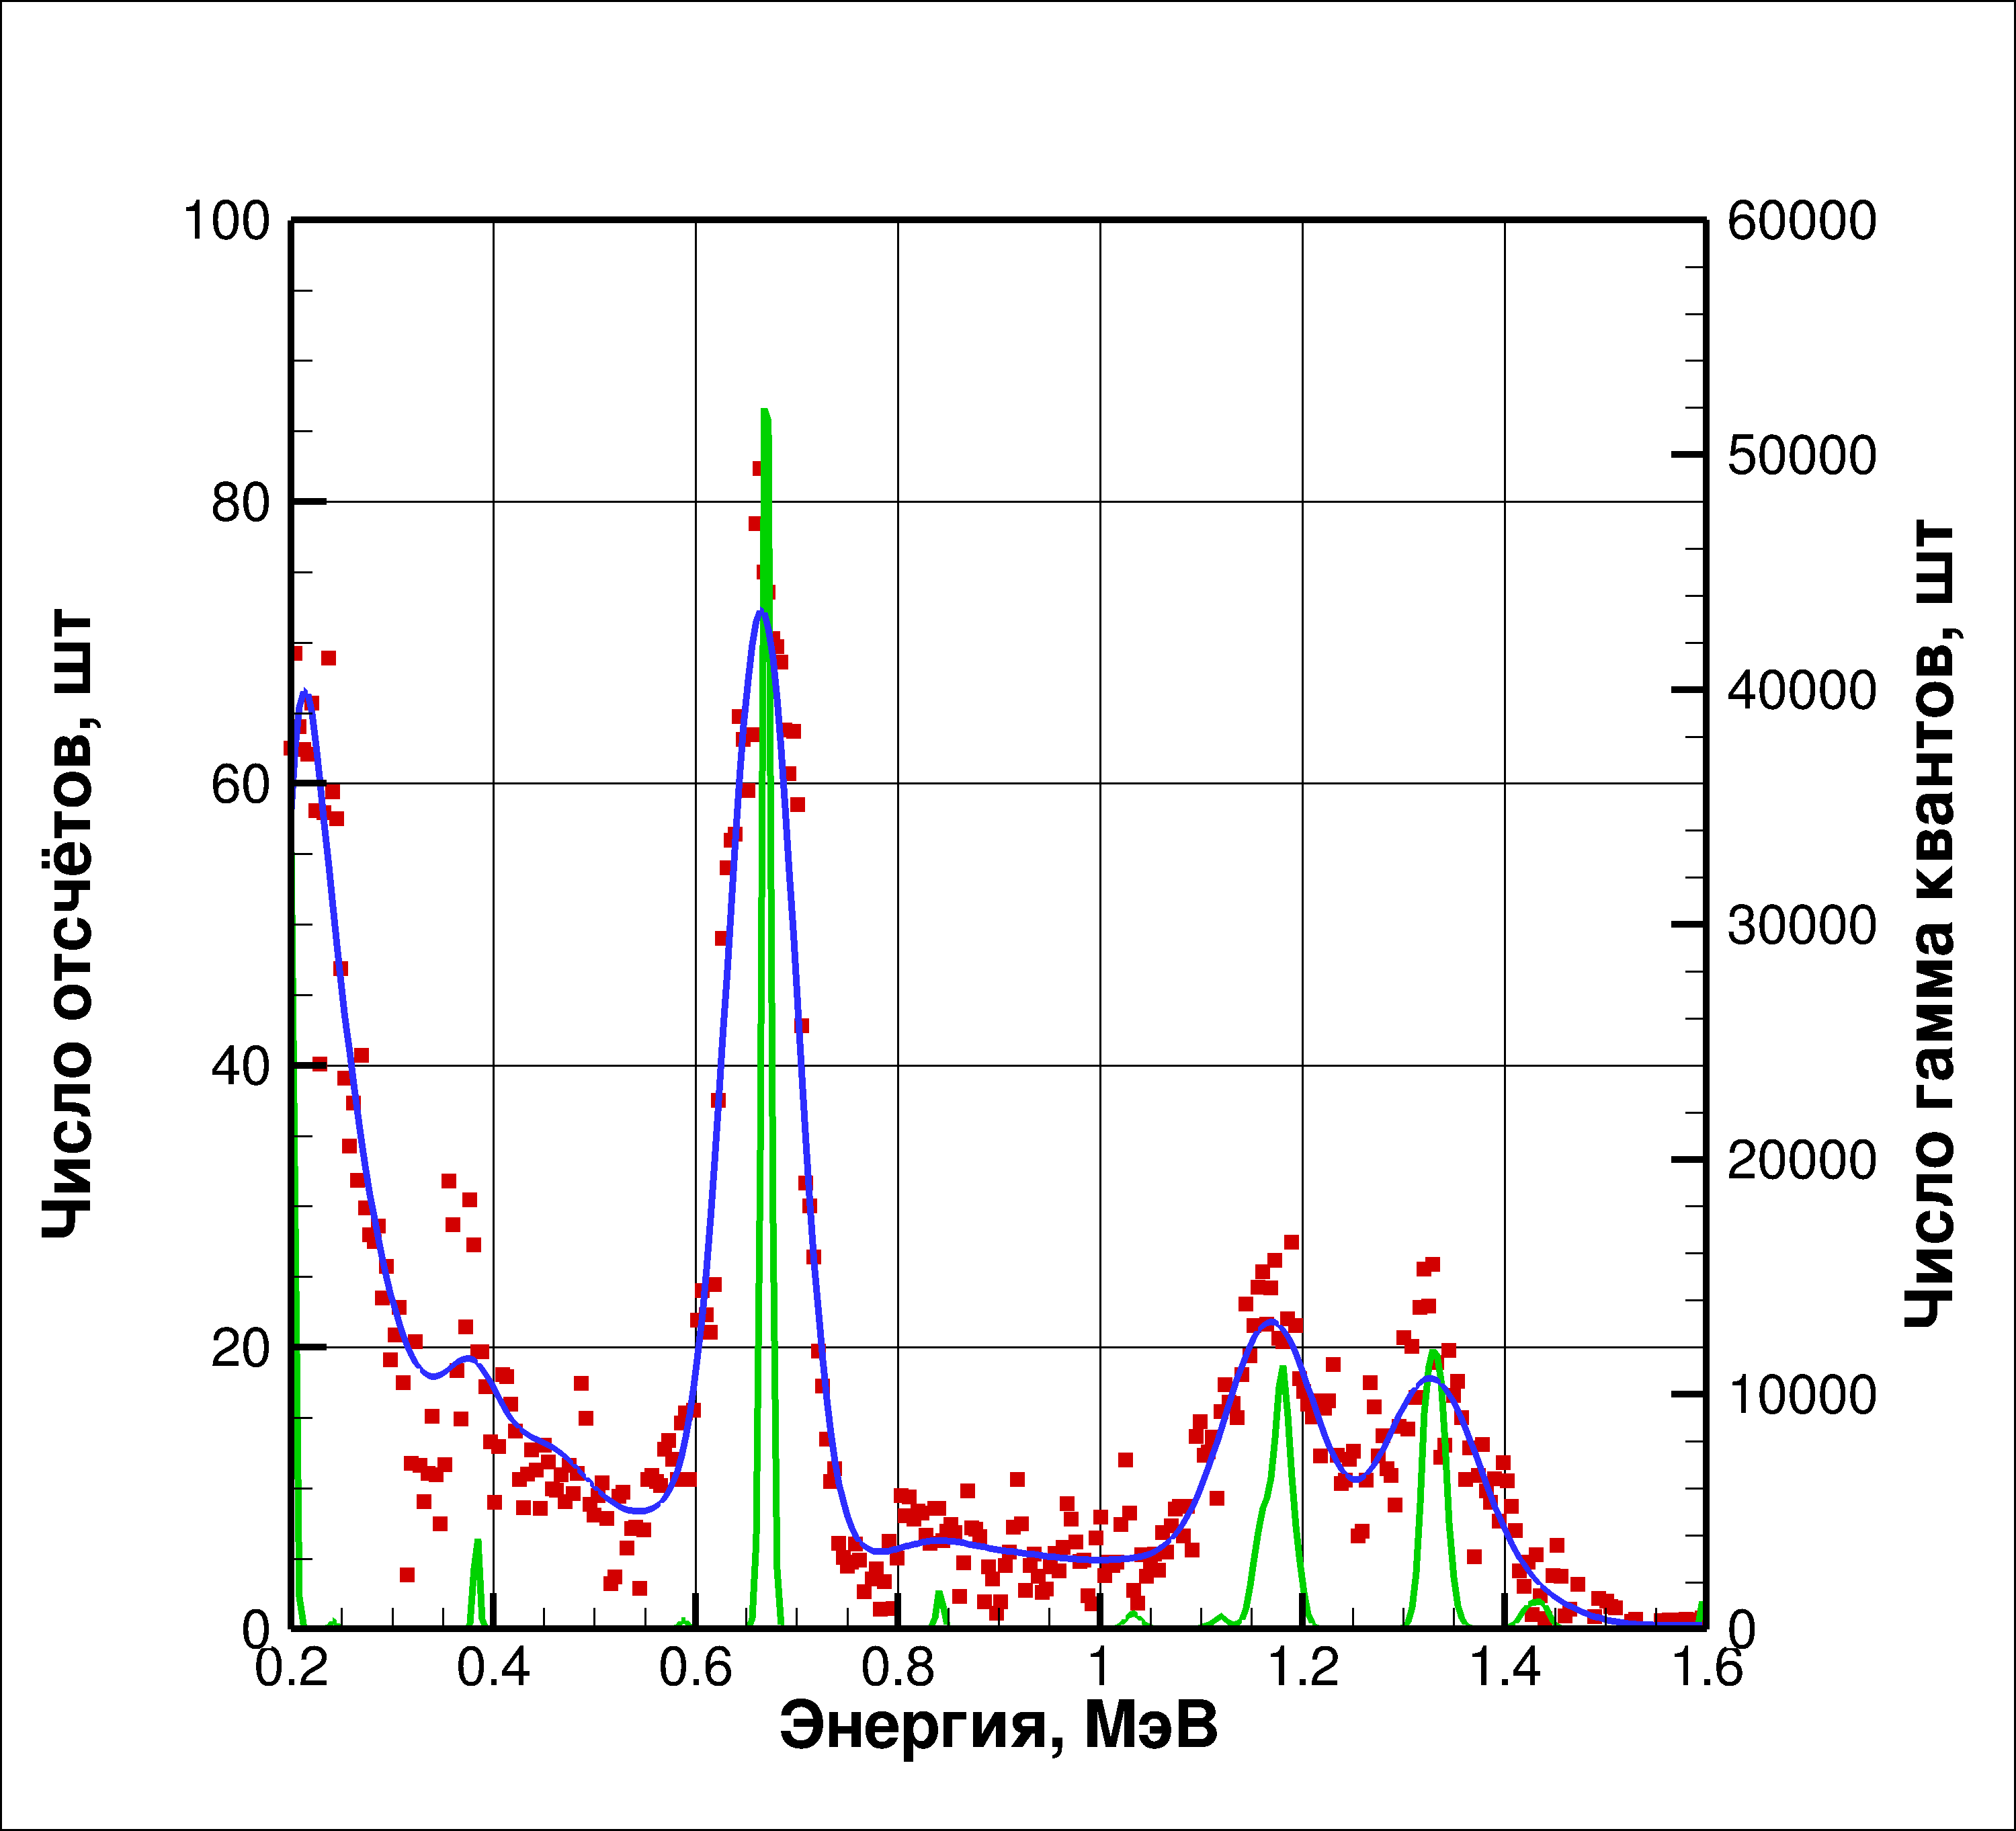
\includegraphics[width=0.52\linewidth]{cocsReconstructIoffe2s} \\ б) \\
    \end{minipage}
    \vspace{5mm}
    \caption{ Спектр источников ${}^{60}$Co и ${}^{137}$Cs, время набора 150 секунд (а) и 2 секунды (б). Красной линией показан измеренный детектором спектр, зелйной линией --- восстановленный спектр источников гамма излучения, синим --- результат <<прямой свёртки>>, интегрирования восстановленного спектра с передаточной функцией детектора (аппаратной функцией с учётом геометрии источника и детектора). В случае идеального восстановления спектра синяя кривая должна совпадать с красными точками.~\cite{Shevelev2013}. }
    \label{fig:cocsReconstructIoffe}
\end{figure}
\FloatBarrier

В другом эксперименте в измерениях использовался тот же самый NaI(Tl) детектор с размерами $\varnothing$150$\times$100~мм. Использовался источник гамма-излучения ${}^{152}$Eu с известной активностью распада. Результат обработки спектра источника ${}^{152}$Eu показан на рисунке~\ref{fig:euReconstructedSpectrum} и в таблице~\ref{tab:euReconstructedLines}. Из этого спектра был предварительно вычтен измеренный спектр фонового излучения. Восстановленный спектр позволил определить все основные линии источника ${}^{152}$Eu. Ошибка определения линий с высокой интенсивностью оказывается сравнительно небольшой. Она может быть объяснена  неточным  определением расстояния до источника. Метод позволил выявить линии с крайне малой интенсивностью 1.212~МэВ, 1.299~МэВ, 0.688~МэВ, 0.586~МэВ, 0.563~МэВ, невидимые в исходном спектре, хотя и с большой относительной ошибкой при определении амплитуды. Удалось обнаружить так же невидимую в исходном спектре линию 0.867~МэВ и сравнительно точно определить её интенсивность. Удалось разрешить близко расположенные пары линий 0.411 и 0.444~МэВ, 1.085 и 1.112~МэВ.~\cite{Khilkevitch2013}

\begin{figure}[ht!]
  \centerfloat{ 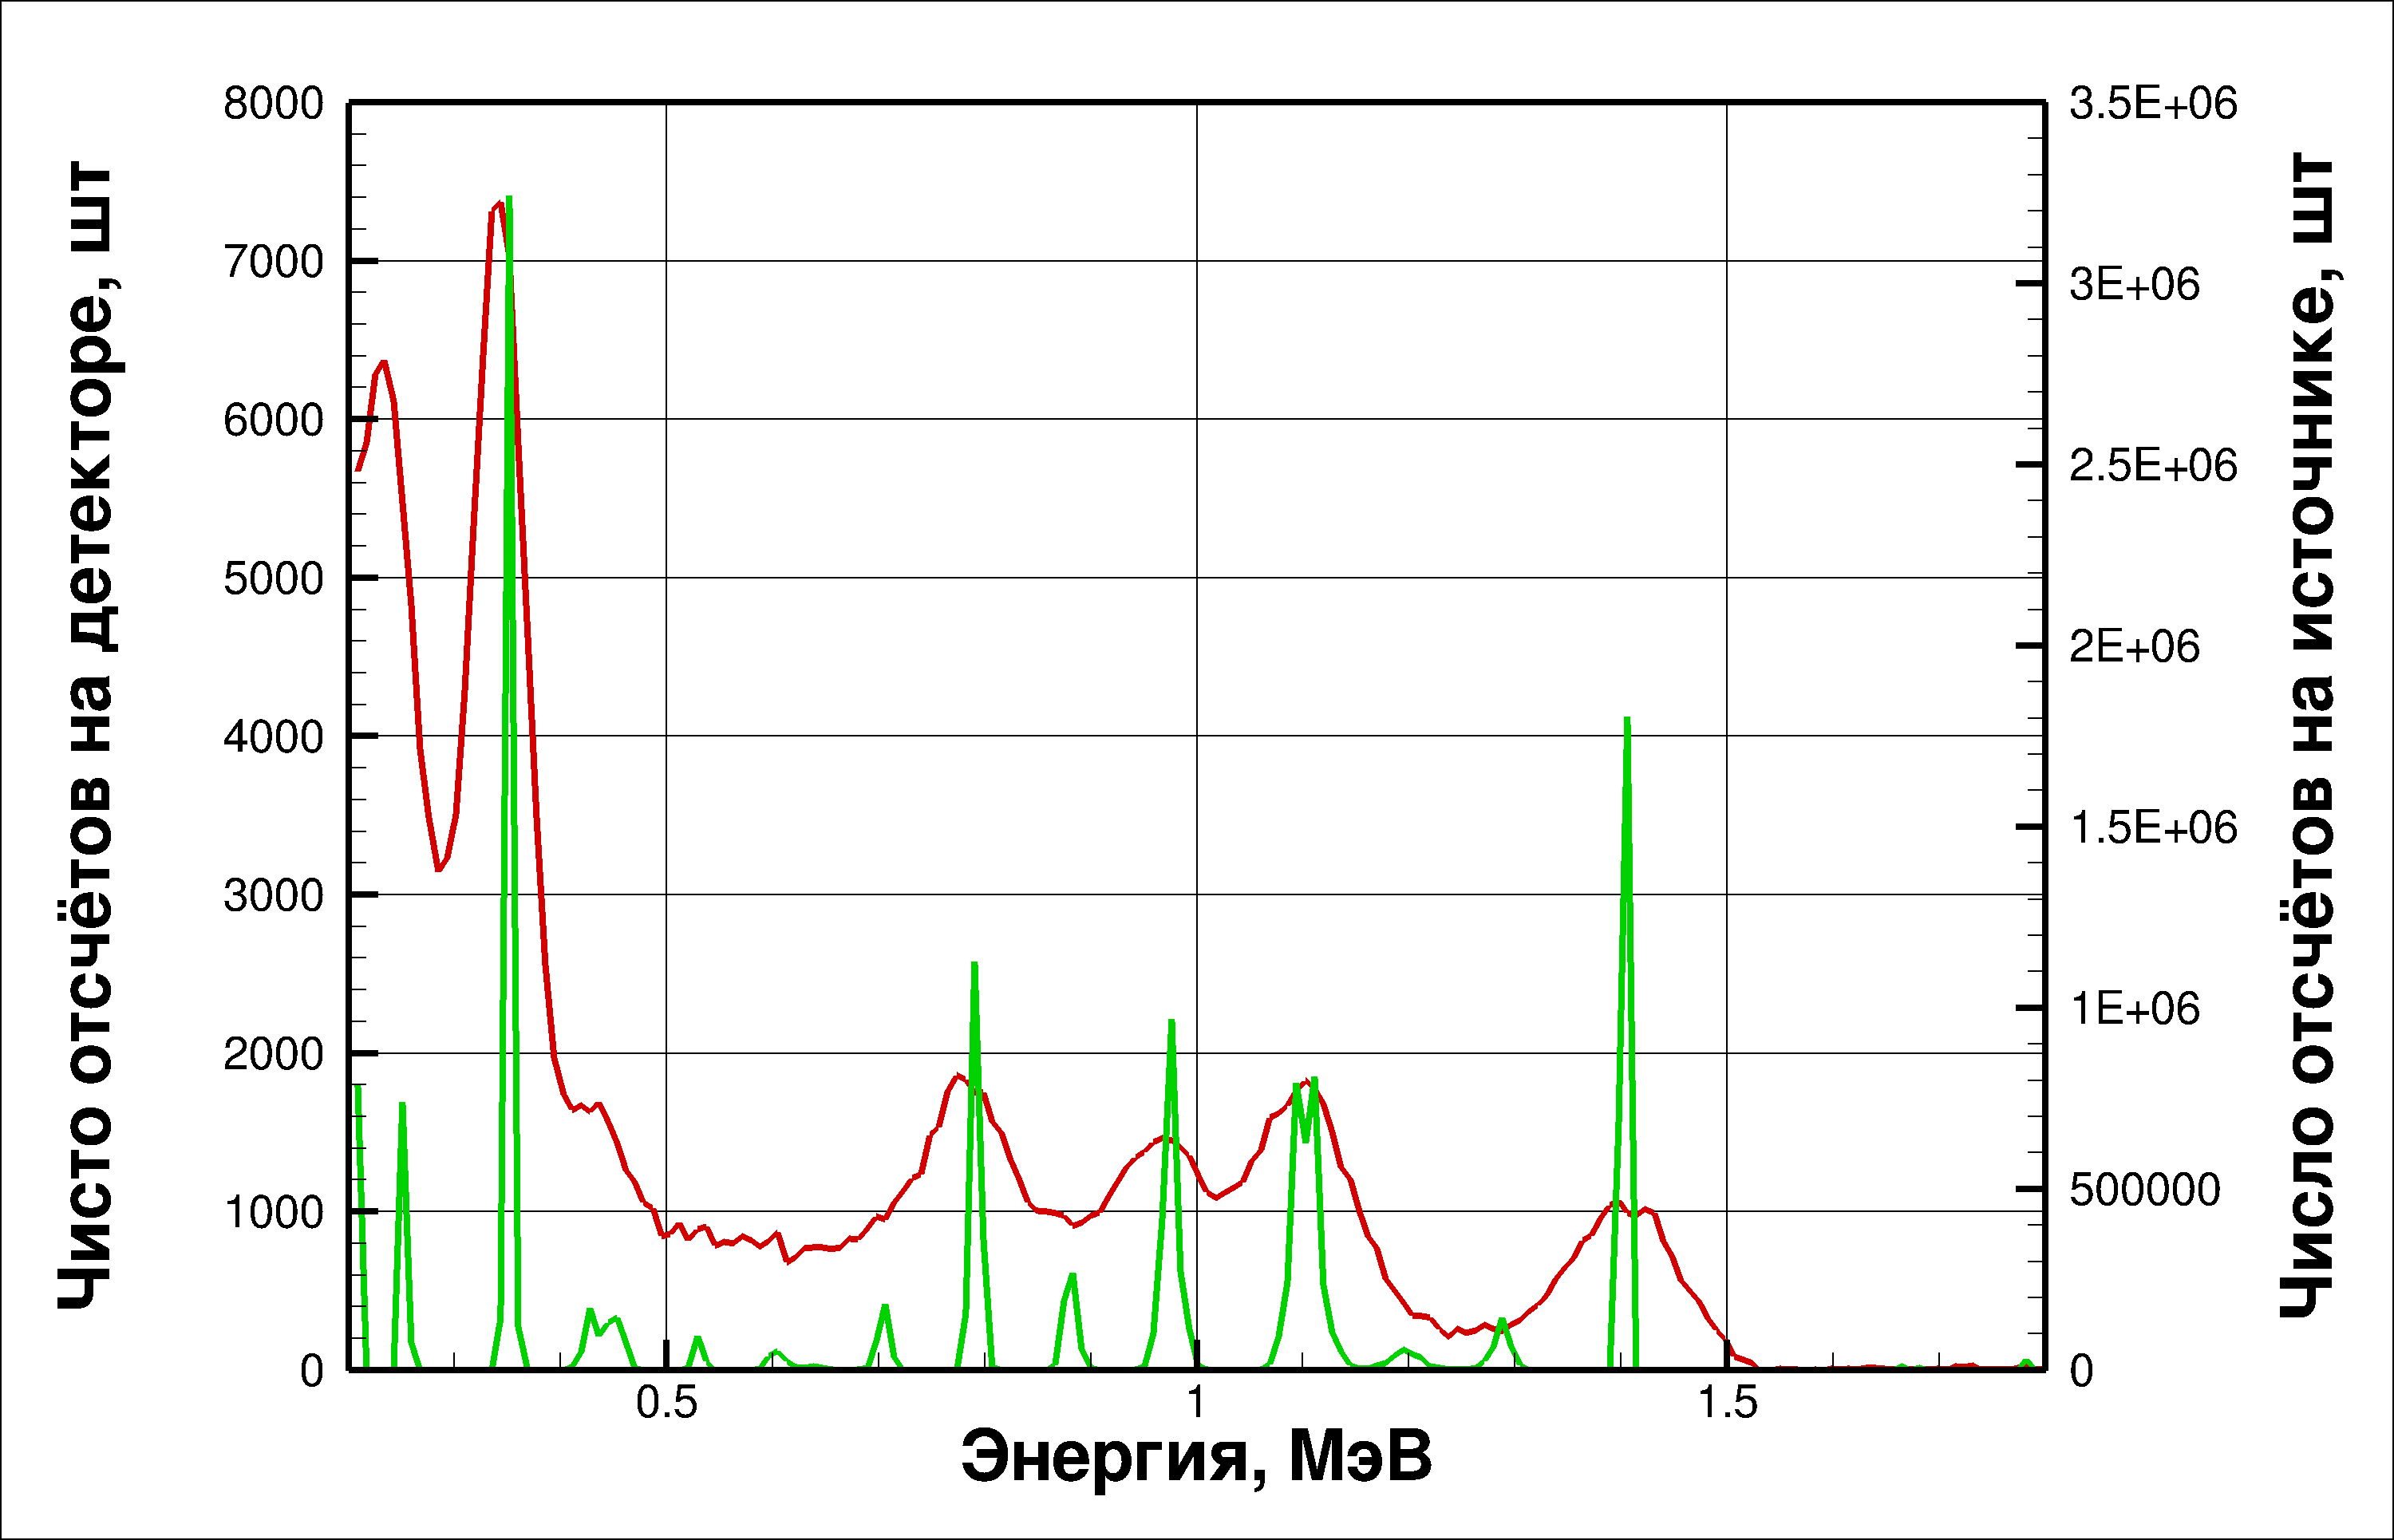
\includegraphics[width=0.52\linewidth]{euReconstructedSpectrum} }
  \caption{ Восстановленный спектр излучения источника ${}^{152}$Eu после вычитания фона. Время набора спектра --- 300 секунд. Красная линия --- измеренный спектр (отсчёты по левой оси), зелёная линия --- восстановленный спектр (отсчёты по правой оси).~\cite{Khilkevitch2013} }
  \label{fig:euReconstructedSpectrum}
\end{figure}

\begin{table}[htbp]
    \centering
    \begin{threeparttable}
      \caption{ Интенсивности и энергии пиков восстановленного спектра источника ${}^{152}$Eu. Интенсивность линий из паспорта представляет собой сумму линий с большой интенсивностью и рядом находящихся линий малой интенсивности (менее 1\%).~\cite{Khilkevitch2013} }
        \label{tab:euReconstructedLines}
        \begin{tabular}{| p{1cm} | p{3.5cm} | p{3.5cm} | p{3.5cm} | p{3.5cm} | }
            \hline
            \makecell{\textnumero} & \makecell{ Энергия линий \\ по паспорту, \\ МэВ } & \makecell{ Энергия \\ восстановлен-\\ных линий, МэВ } & 
                \makecell{Интенсивность \\ по паспорту, c${}^{-1}$} & \makecell{Восстанов-\\ленная \\ интенсив-\\ность, c${}^{-1}$ } \\
            \hline
             1 & 0.245 & 0.243 & 3018 & 2722 \\
             2 & 0.344 & 0.349 & 11115 & 11683 \\
             3 & 0.411 & 0.428 & 945 & 994 \\
             4 & 0.444 & 0.453 & 1269 & 1300 \\
             5 & 0.563 & 0.529 & 447 & 411 \\
             6 & 0.586 & 0.604 & 367 & 441 \\
             7 & 0.688 & 0.706 & 863 & 1033 \\
             8 & 0.778 & 0.790 & 5585 & 5529 \\
             9 & 0.867 & 0.883 & 1841 & 1800 \\
             10 & 0.964 & 0.975 & 6229 & 6316 \\
             11 & 1.085 & 1.035 & 4815 & 4392 \\
             12 & 1.112 & 1.111 & 5501 & 5326 \\
             13 & 1.212 & 1.195 & 673 & 653 \\
             14 & 1.299 & 1.288 & 710 & 1083 \\
             15 & 1.408 & 1.406 & 8469 & 8257 \\
            \hline
        \end{tabular}
    \end{threeparttable}
\end{table}

% ==========================================================

\FloatBarrier
\section{ Восстановление функции распределения убегающих электронов по измеренному спектру излучения }

\subsection{ Использование метода ML-EM для восстановления функции распределения убегающих электронов }

При торможении электрон испускает поток квантов жёсткого рентгеновского излучения, которое может быть зарегистрировано гамма детекторов. Спектр рентгеновского излучения имеет почти непрерывный характер; максимальная энергия рождённых квантов равна кинетической энергии электрона, однако вероятность рождения единственного кванта с максимальной энергией не велика, большая часть спектра излучения приходится на меньшие энергии.~\cite{Kuznetsov1974}

Спектр рентгеновского излучения, генерируемый в процессе торможения электронов, может быть описан следующей формулой:
\begin{equation}
  \label{eq:RunawayConvolution}
  g( \varepsilon ) = \int \limits_0^{ \varepsilon } f(\varepsilon') k( \varepsilon, \varepsilon' ) d \varepsilon'
\end{equation}
где $f(\varepsilon)$ --- функция распределения электронов по энергии, $k( \varepsilon, \varepsilon' )$ --- функция генерации излучения убегающими электронами. Для моноэнергетического пучка электронов с энергией $\varepsilon_0$ и интенсивностью $I$, то есть $ f(\varepsilon) = I \cdot \delta( \varepsilon - \varepsilon_0 ) $, спектр тормозного рентгеновского излучения будет равен $g(\varepsilon) = I \cdot k( \varepsilon, \varepsilon_0 )$. Очевидно что при всех значениях $\varepsilon > \varepsilon'$ значения $k( \varepsilon, \varepsilon' ) = 0$, поскольку электрон не в состоянии сгенерировать гамма квант с энергией больше, чем энергия электрона.~\cite{Shevelev2013} 

Функция $k( \varepsilon, \varepsilon' )$ может быть рассчитана с помощью кода MCNP. Она зависит от угла между линией наблюдения и угловым распределением направления движения электронов, а так же от материала, на котором происходит торможение. Интенсивность излучения оказывается пропорциональна квадрату заряда ядер, на которых происходит рассеяние, а диаграмма углового распределения излучения имеет явно выраженную анизотропию в направлении налетающего пучка электронов.~\cite{Shevelev2013}

Уравнение~\ref{eq:RunawayConvolution} можно подставить в~\ref{eq:BaseConvolution}, тогда:
\begin{equation}
  \label{eq:RunawayBaseConvolution}
  \begin{alignedat}{1}
    s( \varepsilon ) = & \int \limits_0^{+\infty} d \varepsilon' h( \varepsilon, \varepsilon' ) \int \limits_0^{\varepsilon'} d \varepsilon'' f( \varepsilon'') k( \varepsilon', \varepsilon'' ) + n(\varepsilon) \\
    = & \int \limits_0^{+\infty} d \varepsilon'' f( \varepsilon'' ) \int \limits_0^{+\infty} d \varepsilon' h( \varepsilon, \varepsilon' ) k( \varepsilon', \varepsilon'' ) + n(\varepsilon) \\ 
    = & \int \limits_0^{+\infty} d \varepsilon'' f( \varepsilon'' ) h^{tot}( \varepsilon, \varepsilon'' ) + n(\varepsilon)
  \end{alignedat}  
\end{equation}
где $h^{tot}( \varepsilon, \varepsilon'' )$ --- свёртка функций отклика из уравнения~\ref{eq:RunawayConvolution} с передаточной функцией из уравнения~\ref{eq:BaseConvolution}. Вид этого уравнения полностью совпадает с видом уравнения~\ref{eq:BaseConvolution}, и далее для решения уравнения~\ref{eq:RunawayBaseConvolution} можно применять описанный выше метод ML-EM.~\cite{Shevelev2013}

% ----------------------------------------------------------

\subsection{ Проверка корректности восстановления и отработка методики восстановления функции распределения убегающих электронов по энергии }

Если для тестирования процедуры восстановления дискретного спектра можно использовать калибровочные источники гамма излучения, то для тестирования восстановления функции распределения убегающих электронов подобный удобный тестовый объект с известным распределением в нашем распоряжении отсутствует. Поэтому для проверки были использованы сгенерированные и обработаны модельные сигналы.

Для тестирования с помощью кода MCNP с учетом положения детектора NaI(Tl) в Roof lab были рассчитаны спектры тормозного излучения, соответствующие потокам жёсткого рентгена от моноэнергетических электронов в средней плоскости вакуумной камеры токамака JET. Некоторые из этих спектров показаны на рисунке~\ref{fig:mcnpRunawayResponseJetSh2013}. В модели пучок ускоренных электронов с заданным распределением энергии в экваториальной плоскости корпуса JET взаимодействует с объемными ионами. Распределение энергии электронов, используемое в моделировании, показано на рисунке 6(b) зеленой линией с широким пиком в области высоких энергий. Такая форма распределения вполне реальна при наличии первичных и вторичных механизмов генерации УЭ, а также в условиях, ограничивающих неуправляемый рост энергии, например, за счет потерь на синхротронное излучение [22]. Смоделирован спектр ЖРИ, который мог быть зарегистрирован детектором NaI(Tl) с распределением статистики Пуассона. Он показан на рис. 6(с) черными точками. После этого применяется процедура деконволюции. Результат показан на рис. 6(b) красной пунктирной линией. Результат свертки полученного распределения электронов с функцией отклика детектора представлен на рисунке 6(c) синей пунктирной линией. Расчеты проводились в вакуумной геометрии JET для дейтериевой плазмы с плотностью электронов 5 · 1019 м−2 и 2\% примеси углерода. Интеграл по полученному распределению равен числу электронов, прошедших через видимый объем плазмы.
детектором во время сбора спектра. В измеренном спектре предполагалась статистика Пуассона. х 2 теста
дал следующие результаты: χred 2
 = 0,6 для спектров ЖРИ.
Для модели и полученных распределений электронов χred
 2
 = 0,71.

\begin{figure}[ht!]
  \centerfloat{ 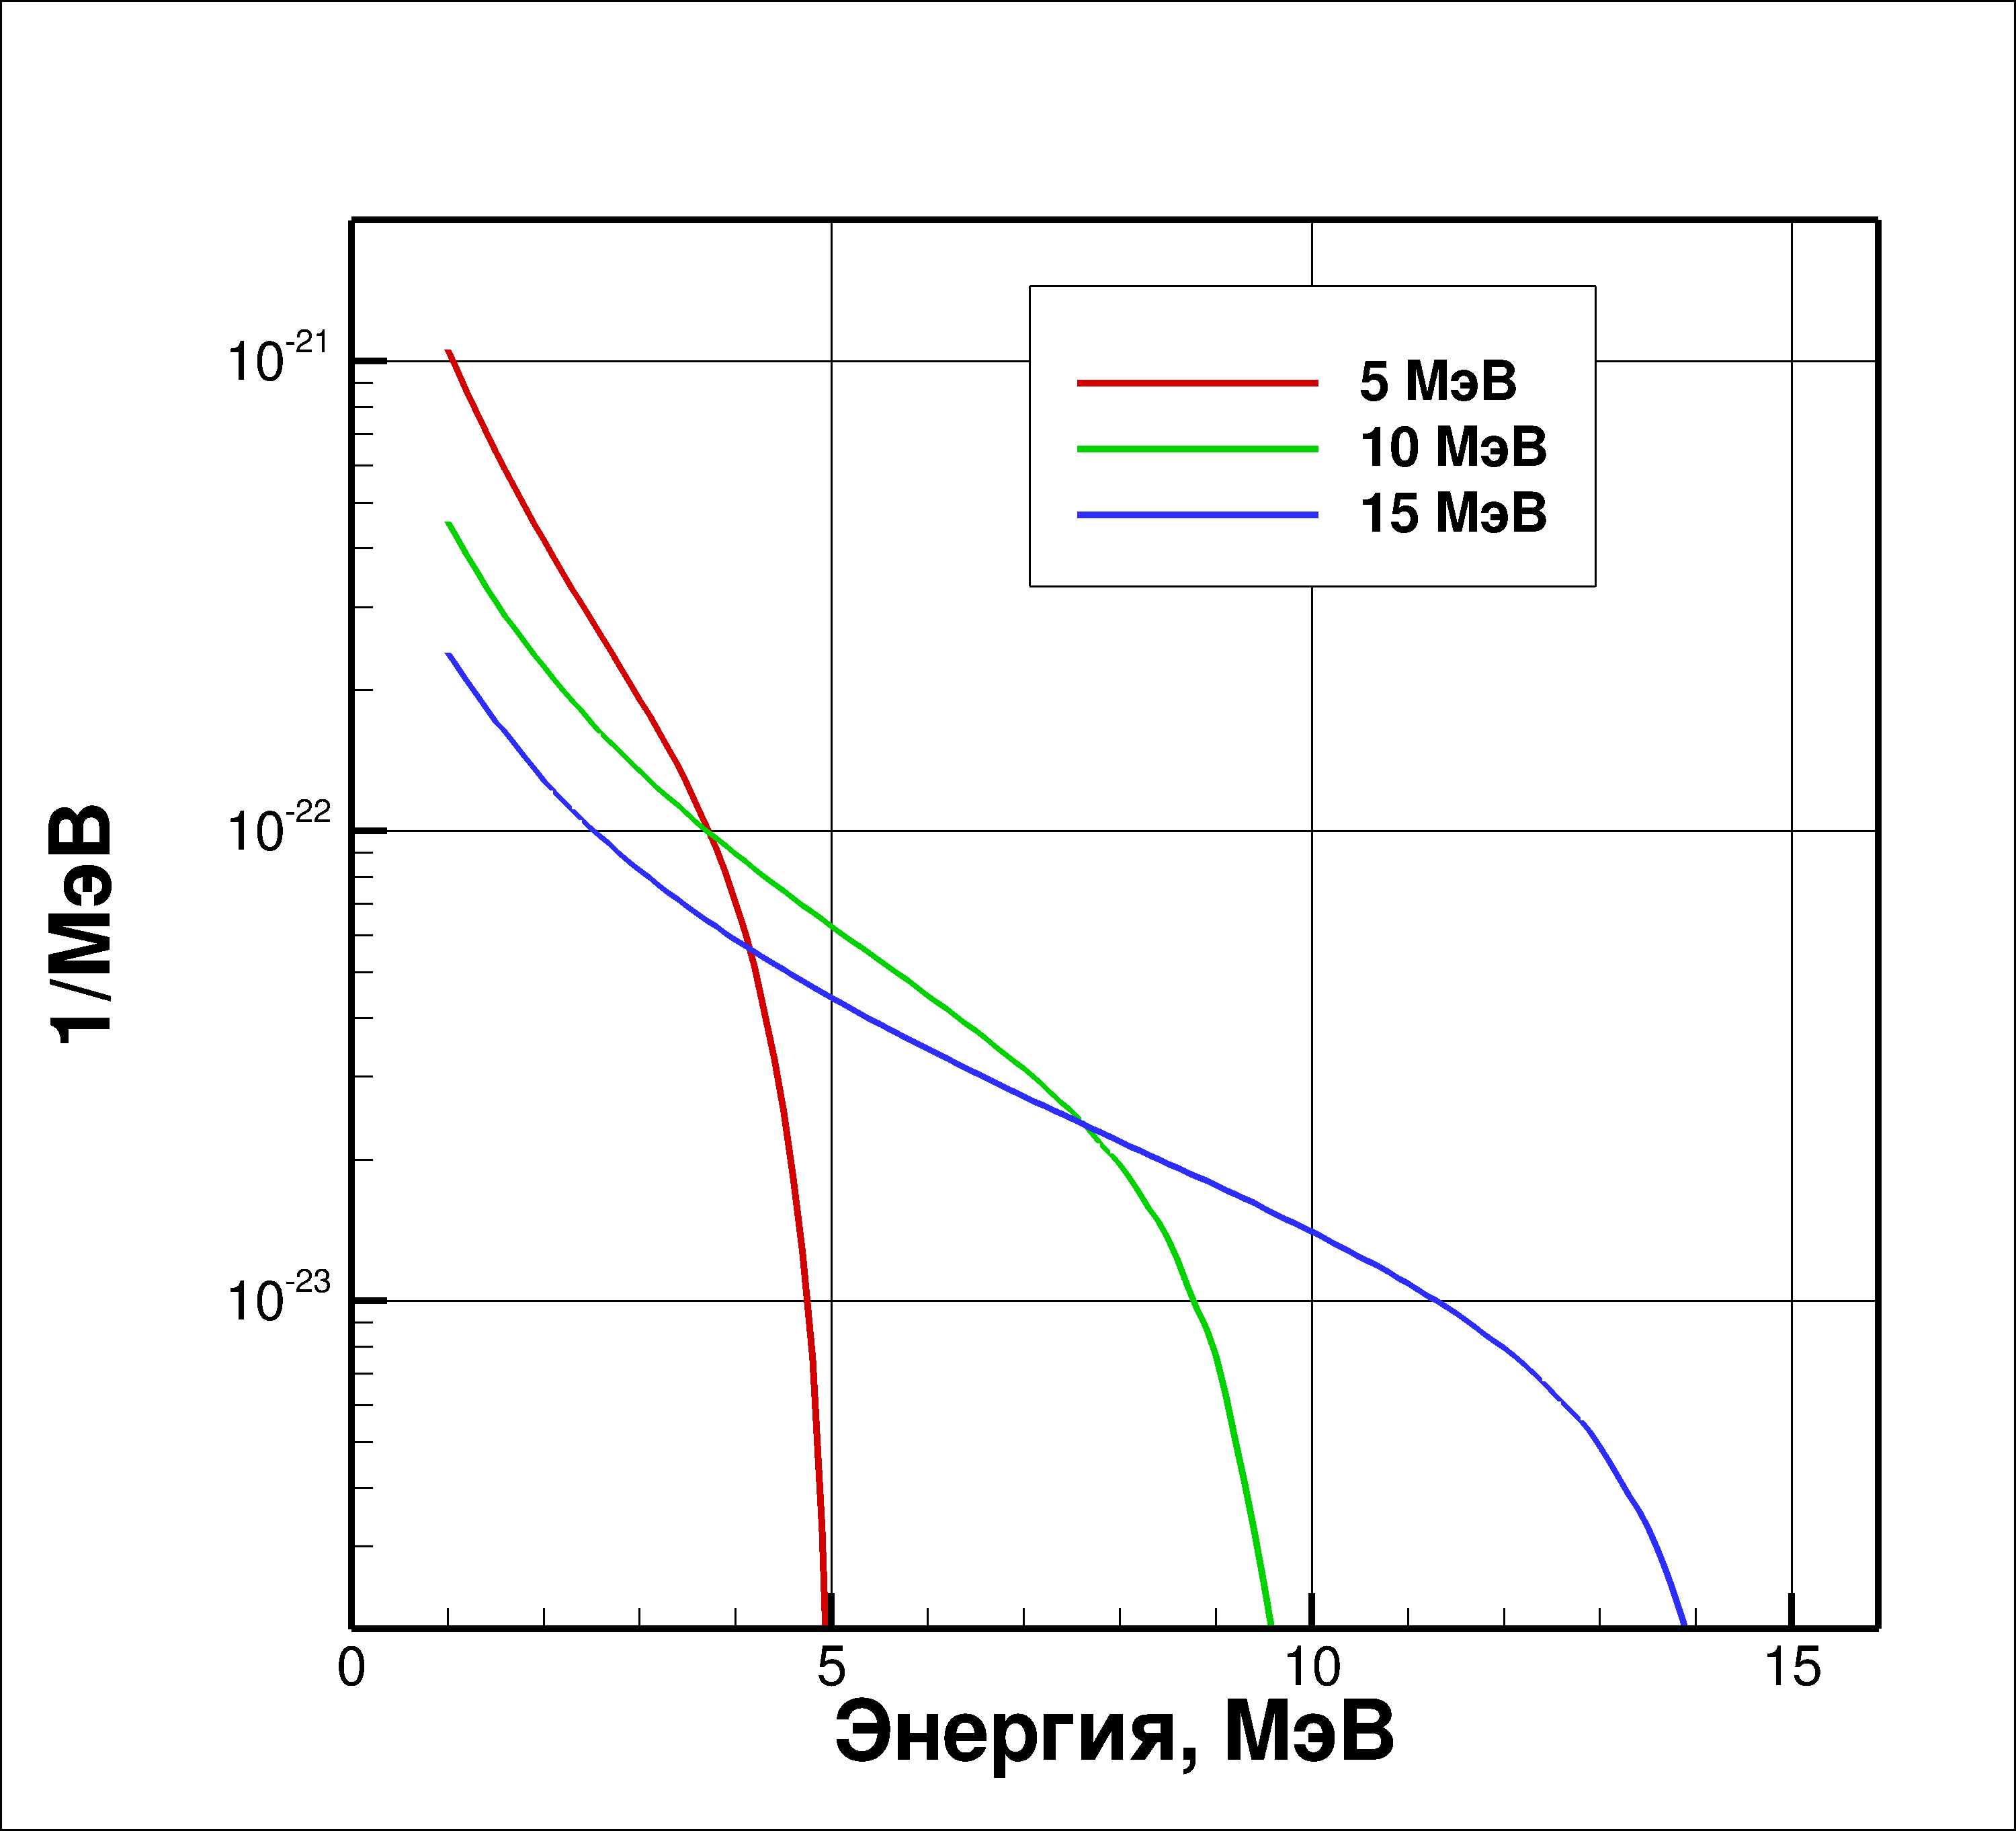
\includegraphics[width=0.52\linewidth]{mcnpRunawayResponseJetSh2013} }
  \caption{ Спектры жёсткого рентгеновского излучения, генерируемые убегающими электронами с энергиями 5, 10, 15~МэВ, рассчитанные с помощью кода MCNP. Расчёт проведён для условий токамака JET.~\cite{Shevelev2013} }
  \label{fig:mcnpRunawayResponseJetSh2013}
\end{figure}


Восстановленное распределение электронов продемонстрировало очень близкое совпадение с модельным спектром и дало максимальную энергию 11 МэВ с очень высокой точностью, в то время как измерения HXR дали 10 МэВ. В реальных измерениях HXR высокоэнергетический диапазон спектра HXR может иметь очень плохую статистику: единичные отсчеты на канал или полное отсутствие событий. Причинами этого являются ограниченное время набора спектра и ограничение нагрузочных характеристик детектора. Детекторы имеют мертвое время при регистрации гамма-излучения, что приводит к потерям событий и ограничению максимальной скорости счета. Максимально достижимая скорость счета зависит от свойств кристалла и электронной схемы. Алгоритм ML-EM использует информацию из «видимой» части спектра для восстановления функции распределения в каждом


% ==========================================================

\FloatBarrier
